\documentclass[10pt]{beamer}

% \usepackage[utf8]{inputenc}
% \usepackage[T1]{fontenc}
% \usepackage{amsfonts}

\usetheme[progressbar=frametitle]{metropolis}
\usepackage{appendixnumberbeamer}

\usepackage{booktabs}
\usepackage[scale=2]{ccicons}

\usepackage{pgfplots}
\usepgfplotslibrary{dateplot}

\usepackage{xspace}
\newcommand{\themename}{\textbf{\textsc{metropolis}}\xspace}

%%%%%%%%%%%%%%%%%%%%%%%%%%%%%%%%%%%%%%%%%%%%%%%%%%%%%%%%%%%%%%%%%%%%%%
% CATEGORY THEORY
\newcommand\newterm[2][]{\textbf{\itshape\color{blue!50!black}#2}}
\newcommand{\cat}[1]{\mathcal{#1}}      % Arbitrary category
\newcommand{\scat}[1]{\mathbf{#1}}      % Arbitrary small category
\newcommand{\ob}[1]{\mathbf{ob}(#1)}       % Objects of a category
\newcommand\id{\mathsf{id}}

\DeclareRobustCommand{\step}{\bigskip\noindent}

\newcommand{\abs}[1]{\left\vert #1 \right\vert}
\newcommand{\norm}[1]{\lVert #1 \rVert}
\newcommand{\dom}[1]{\mathbf{dom}\left(#1\right)}
\newcommand{\range}[1]{\mathbf{range}\left(#1\right)}
\newcommand\N{\mathbb{N}}

%%%%%%%%%%%%%%%%%%%%%%%%%%%%%%%%%%%%%%%%%%%%%%%%%%%%%%%%%%%%%%%%%%%%%%

\title{Turing Categories \& Computability}
\subtitle{An abstract look at computability}
\date{\today}
% \date{}
\author{Amittai Siavava}
\institute{Dartmouth Math 29}
% \titlegraphic{\hfill\includegraphics[height=1.5cm]{logo.pdf}}

\begin{document}

\maketitle

\begin{frame}{Table of contents}
  \setbeamertemplate{section in toc}[sections numbered]
  \tableofcontents%[hideallsubsections]
\end{frame}

\section[Categories]{Category Theory}

\subsection{Motivation}

\begin{frame}[fragile]{What is Category Theory Anyway?}

  You may have noticed that different branches of mathematics
  seem to share similar structures and, sometimes, even results.
  

  \step
  \begin{figure}[H]
    \centering
    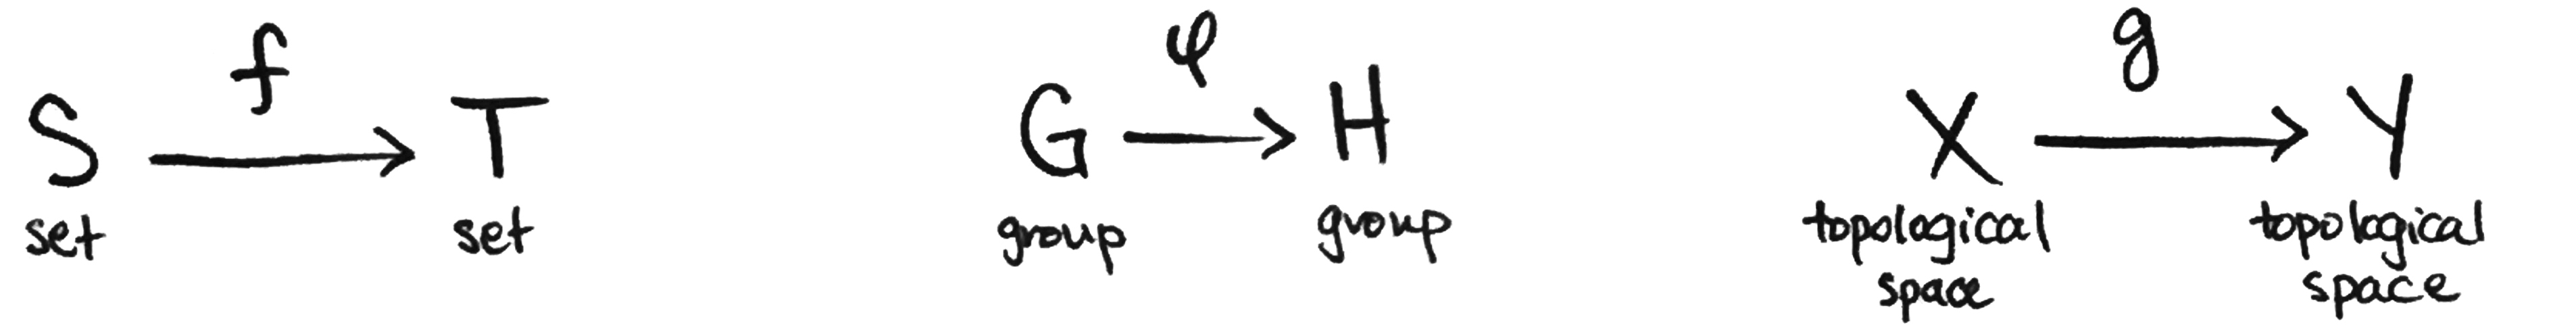
\includegraphics[width=\textwidth]{res/parallels.jpeg}
    \caption{sets, groups, spaces...}
  \end{figure}
  
  Can these similarities and differences teach us anything... \\
  ...at all... \\
  about these structures?
\end{frame}

\subsection{Categories}

\begin{frame}[fragile]{What is Category Theory Anyway?}
  \begin{definition}

    \step
    A \newterm{category} $\cat{C}$ consists of:
    \begin{enumerate}
      \item A collection $\ob{\cat{C}}$ of \newterm{objects};
      \item For each pair of objects $A, B \in \ob{\cat{C}}$,
        a set $\cat{C}(A,B)$ of \newterm{morphisms} (aka ``\newterm{arrows}'') from $A$ to $B$;
      \item For each object $A \in \ob{\cat{C}}$, a morphism $\id_A \in \cat{C}(A,A)$;
      \item For each triple of objects $A, B, C \in \ob{\cat{C}}$,
        a composition function
        \[
          \circ : \cat{C}(B,C) \times \cat{C}(A,B) \to \cat{C}(A,C).
        \]
    \end{enumerate}
    \step
    ...preserving associativity: $\qquad f \circ (g \circ h) = (f \circ g) \circ h$

    ...and identity: $\qquad \id_B \circ f = f = f \circ \id_A$.
  \end{definition}

\end{frame}

\begin{frame}[fragile]{Categories... Examples?}

  % create table of category name -> objects -> morphisms -> composition -> identity
  \begin{figure}[H]
    \centering
    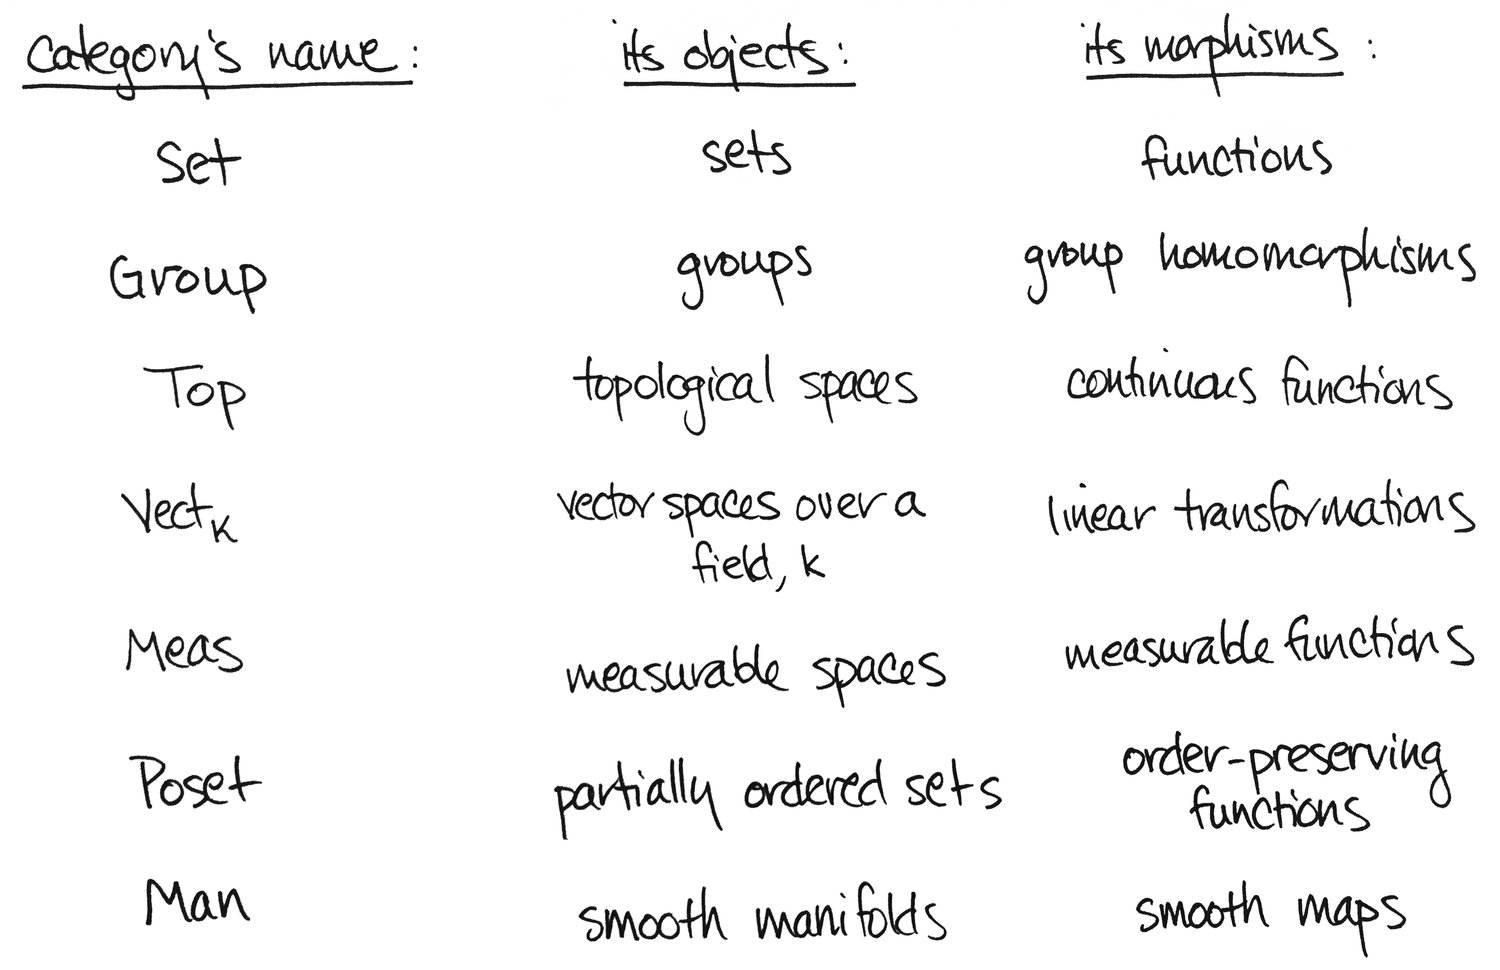
\includegraphics[width=\textwidth]{res/category-examples.jpeg}
  \end{figure}

\end{frame}

% \begin{frame}[fragile]{Categories... Examples?}

%   % create table of category name -> objects -> morphisms -> isomorphism -> composition
%   \begin{table}[H]
%     \centering
%     \begin{tabular}{|c|c|c|c|c|}
%       \hline
%       Category & Objects & Morphisms & Isomorphisms \\
%       \midrule
%       $\mathsf{Set}$ & Sets & Functions & Bijections \\
%       $\mathsf{Grp}$ & Groups & Group homomorphisms & Isomorphisms \\
%       $\mathsf{Top}$ & Topological spaces & Continuous functions & Homeomorphisms \\
%       $\mathsf{Vect}_k$ & Vector spaces over $k$ & Linear transformations & Isomorphisms \\
%       $\mathsf{Pos}$ & Partially ordered sets & Order-preserving functions & Order isomorphisms \\
%       $\mathsf{Cat}$ & Categories & Functors & Natural isomorphisms \\
%       \hline
%     \end{tabular}
%   \end{table}

% \end{frame}

\subsection{Functors}

\begin{frame}[fragile]{Category Theory is all about Relationships!}
  Category theory strips away \emph{a lot} of detail. \newline
  By ignoring the details, attention is diverted to
  \textbf{relationships} between objects and morphisms.

  % functor definition
  \begin{definition}

    \step
    A \newterm{functor} $F : \cat{C} \to \cat{D}$ between categories $\cat{C}$ and $\cat{D}$
    consists of:
    \begin{enumerate}
      \item A function $F : \ob{\cat{C}} \to \ob{\cat{D}}$;
      \item For each pair of objects $A, B \in \ob{\cat{C}}$, a function
        \[
          F : \cat{C}(A,B) \to \cat{D}(F(A), F(B)).
        \]
    \end{enumerate}
    ...preserving composition and identity.
  \end{definition}
\end{frame}

\begin{frame}[fragile]{Functors... Examples?}

  % create table of category name -> objects -> morphisms -> composition -> identity
  \begin{figure}[H]
    \centering
    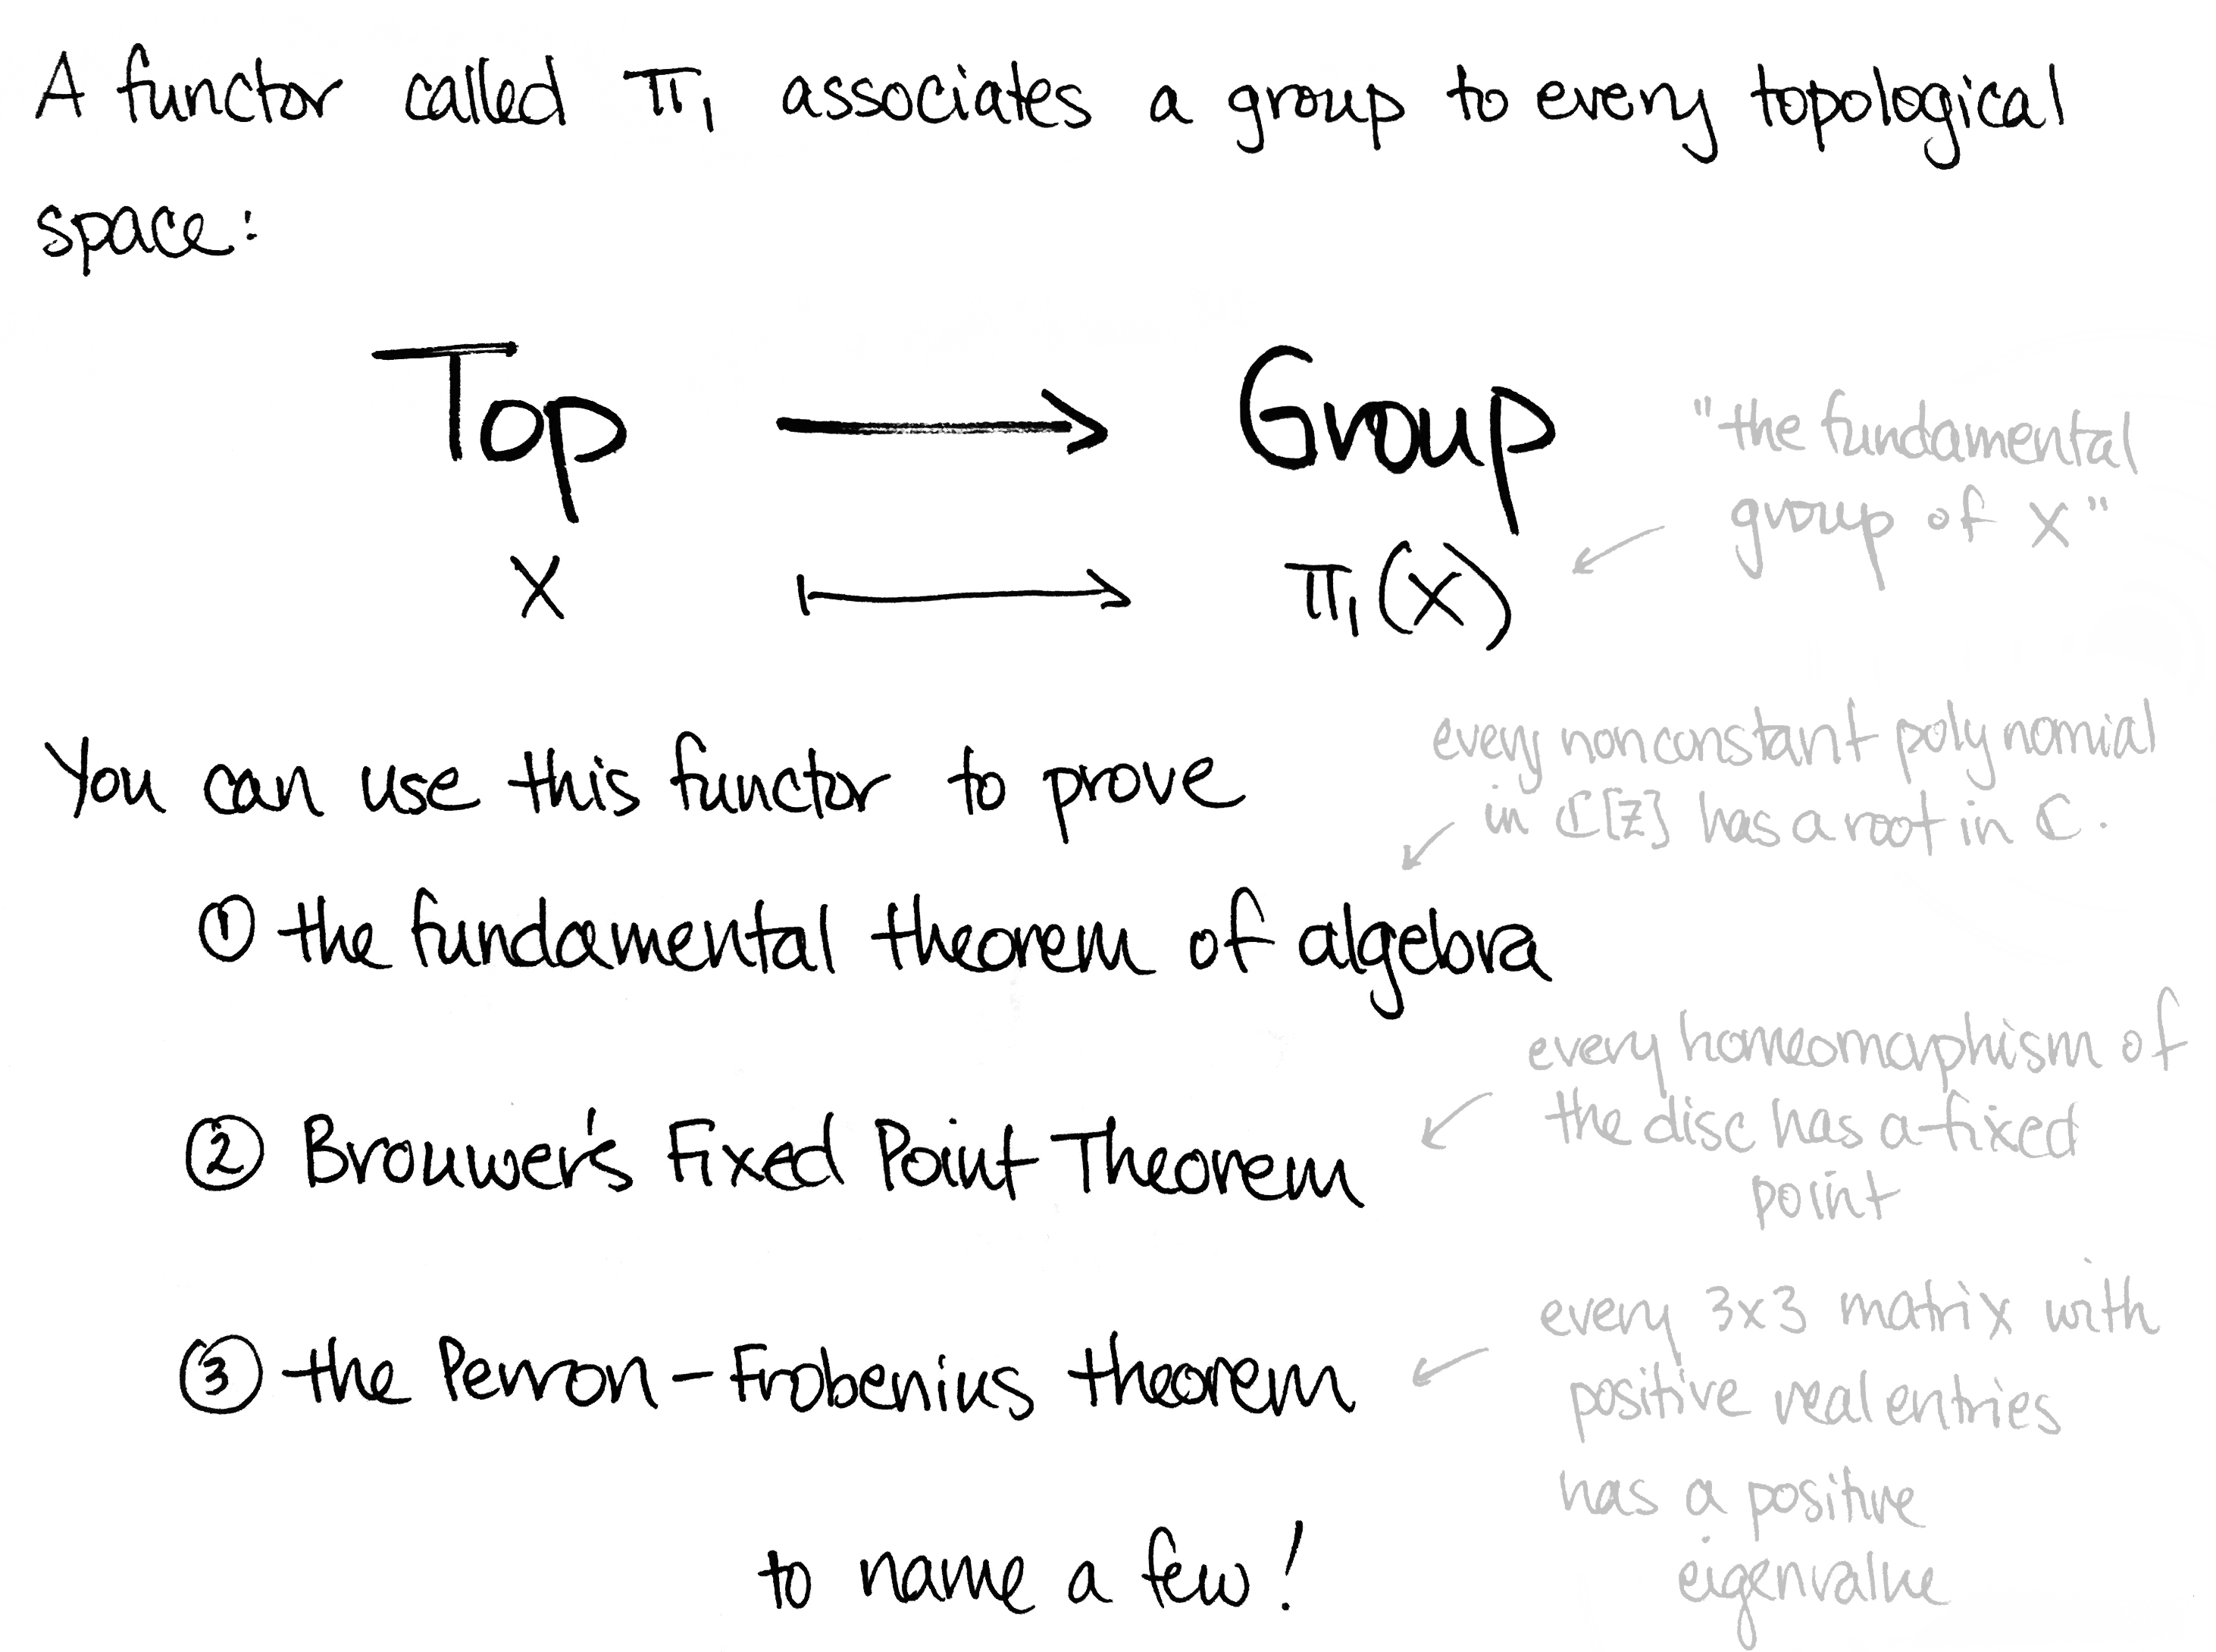
\includegraphics[width=\textwidth]{res/top-group-functor.jpeg}
  \end{figure}

\end{frame}

\section{Turing Categories}

\begin{frame}[fragile]{Turing Categories?}

  % create table of category name -> objects -> morphisms -> composition -> identity
  Are you saying that... \\
  \qquad If you put codes for Turing machines in a... \\
  \qquad \qquad thing... \\
  
  \step
  you get a category?

  We need to address a few things.

  \begin{enumerate}
    \item \alert{morphisms}? or \alert{objects}?
    \item \alert{partiality}?
    \item \alert{what about the system of coding}?
  \end{enumerate}

\end{frame}

\subsection{Turing Structure}

\begin{frame}[fragile]{Yes, Turing Categories!}

  \alert{But we need some more structure}

  Specifically, we need:
  \begin{enumerate}
    \item A \newterm{restriction structure} to handle partiality; \newline
      \emph{
        Assigns to each morphism $f : A \to B$ a morphism
        $\bar{f} : A \to \dom{A} \subseteq A$
        (such that a few properties hold).
      }
    \item A \newterm{Turing object} $T$ as some kind of coding context
      for programs (turing machine, register machine, finite automata, etc.)
    \item A universal \newterm{application morphism} $\tau_{X,Y} : T \times X \to Y$
      that represents the application of a program (in $T$) to data (in $X$)
      to produce a result (in $Y$).
    \item objects defined to $\N$, $\N^2$, $\N^3$, and so on...
    \item morphisms defined to be the codings of partial computable functions.
  \end{enumerate}

\end{frame}

\subsection{Examples}

\begin{frame}[fragile]{Yes, Turing Categories.}

  % create table of category name -> objects -> morphisms -> composition -> identity
  Yes, we're saying that if you put... \\
  \qquad codes for \alert{machines} (consistent Turing object!) as \alert{morphisms} \\
  \qquad \qquad appropriate domains and codomains as \alert{objects} \\
  \qquad \qquad \qquad enforce partiality with a \alert{restriction structure} \\
  \qquad \qquad \qquad \qquad define $\tau(e, n) = \varphi_e(n)$ \\
  
  \step
  \alert{you get a category}!

\end{frame}

\begin{frame}[fragile]{Yes, Turing Categories.}

  % create table of category name -> objects -> morphisms -> composition -> identity
  more interesting categories if you...
  
  \begin{enumerate}
    \item restrict to unary, binary, ternary functions, etc.
    \item define each $f : \N^k \to \N^m$ to be a $k$-ary function
      that applies $m$ $k$-ary functions in parallel.
      (\alert{in some cases, this somewhat reproduces linear algebra}).
  \end{enumerate}

  \step
  You can also show that much of what we know about computability
  ($s-m-n$, recursion, etc.) holds in this abstract setting.
  \emph{
    In some cases, something breaks --- and that can also tell us
    something about computability.
  }

  References
  ~\cite{APPLICATIVE-STRUCTURES,BRADLEY,TURING-CATEGORIES,CATEGORY-THEORY-TEXT}

\end{frame}

{\setbeamercolor{palette primary}{fg=black, bg=yellow}
\begin{frame}[standout]
  Questions?
\end{frame}
}

\appendix

% \begin{frame}[fragile]{Backup slides}
%   Sometimes, it is useful to add slides at the end of your presentation to
%   refer to during audience questions.

%   The best way to do this is to include the \verb|appendixnumberbeamer|
%   package in your preamble and call \verb|\appendix| before your backup slides.

%   \themename will automatically turn off slide numbering and progress bars for
%   slides in the appendix.
% \end{frame}

\begin{frame}[allowframebreaks]{References}

  \bibliography{presentation}
  \bibliographystyle{abbrv}

\end{frame}

\end{document}
